\chapter{Approach}
In this chapter, I will outline how my thesis will be realized and provide source code that can be merged into the LiSSA project.
My work aims to implement three different classifiers into the framework.
First, I plan to implement a simple \ToT classifier in \autoref{approach:sec:tot} to broaden the baseline to compare later optimized prompts against.
Next, I expect to work on a reduced iterative optimizer in \autoref{approach:sec:naive_iterative} using a naive approach to optimization.
After this already provides basic components and data to evaluate the more sophisticated algorithm by \citewithauthor{pryzant2023AutomaticPrompt} will be implemented in \autoref{approach:sec:gradient_descent}.
Last but not least, I will explain how I plan to evaluate and compare my findings in \autoref{approach:sec:evaluation}.

\section{Simple Tree-of-Thought Classifier}
\label{approach:sec:tot}

\begin{figure}
    %TODO: replicate this figure!
    \centering
    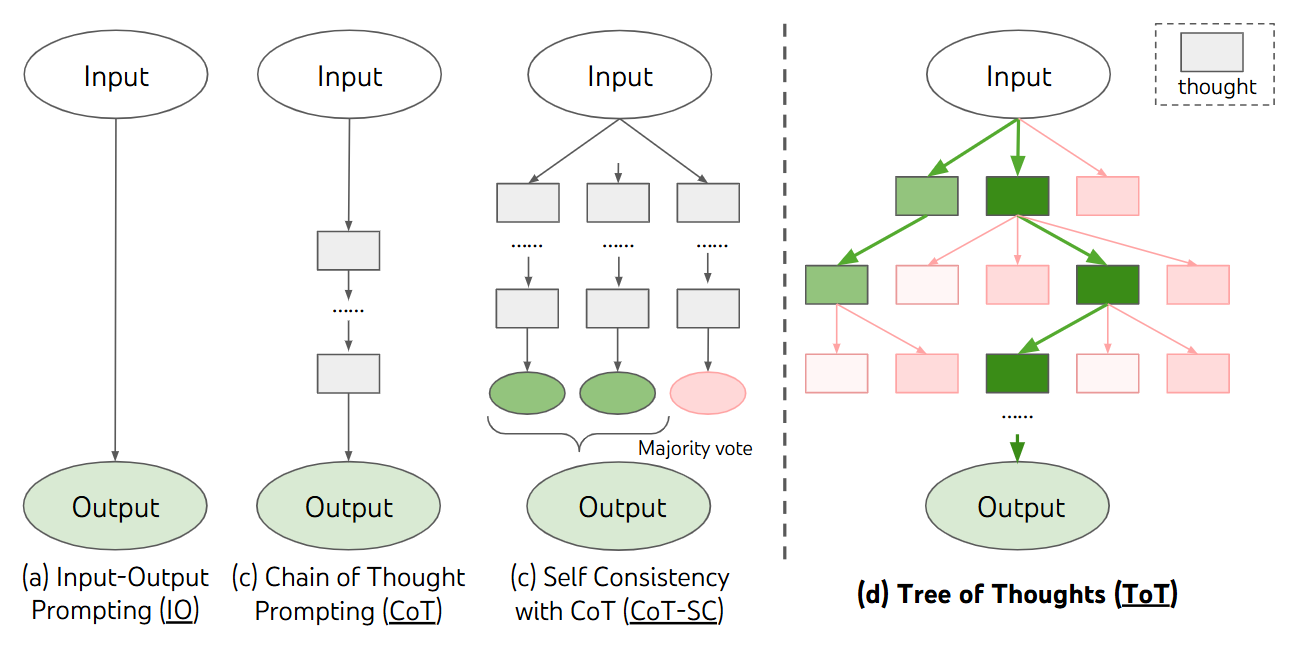
\includegraphics[width=\linewidth]{graphics/ToT_Yao}
    \caption{Tree of Thought visualization by \citewithauthor{yao2023TreeThoughts}}
    \label{fig:ToT_visualization}
\end{figure}

\Ac{ToT} is a prompting technique exploring more different branches of thoughts than typical \CoT prompts.
As illustrated in \autoref{fig:ToT_visualization}, many branches are explored concurrently instead of following a single strain of thoughts like \CoT prompting.
The prompts by \citewithauthor{hulbert2023UsingTreeofThought} aim to simplify \ToT prompting into a singular request, instead of chaining multiple calls.
I will use one of their prompts.
The benchmark data to compare \ToT prompting with the existing zero-shot and \CoT classifiers also exists in public repositories~\cite{fuchss2022ArDoCoBenchmark, hey2025ReplicationPackage}.

The LiSSA framework is publicly accessible in a repository using the MIT license. Various classifiers are already included there.
They can be used as an inspiration for development.
The class \verb|classifier| is an abstraction of all classifiers.
It provides basic functionality to include further classifiers.
Integration for different \LLM providers, such as Chat-GPT, Ollama, and Blablador, already exists in the framework.
The new classifier can be plugged in directly with little more effort than writing the request prompt and implementing the \verb|classify| function to extract the classification result out of the \LLM output.

This work package has two major goals.
Foremost, to get confident and set up with the general project structure and benchmark data.
This will be a prerequisite for all future work in the LiSSA framework.
Second, this will broaden the baseline to compare later results and possible improvements against.




\section{Naive Iterative Optimizing Classifier}
\label{approach:sec:naive_iterative}
Another classifier implementation will be the simplest automatic iterative prompt optimization algorithm.
The same existing abstract \verb|classifier| class can be used as in \autoref{phase_initial_overview} to provide basic functionality for the iteratively optimized classifier.

Next, a function $f$ will be required to quantify the result, also referred to as performance, of the current prompt $p$ iteration, called to a large language model $llm$ using a set of training data $X$.
The simple approach here is to use the successful retrieval rate by dividing the number of correctly classified trace links by the total number of recoverable trace links.
The function $f$ will need to have the same range for any set of training data to ensure the threshold value $t$ will always be viable.

\begin{align}
        f: llm(p, X) \rightarrow [0, 1] \\
        t \in [0, 1]
\end{align}

The benchmark data by \citewithauthor{hey2025ReplicationPackage} also provides the gold standard for each given problem.
The total amount of recoverable trace links is thus already available. 
%\textit{to-do: how can the task set be divided into training and testing data? Use one entire TLR problem for training, the remaining for testing?}

To improve the performance, an optimization prompt is used.
As visualized in \autoref{fig:iterative_core_loop} the expected outputs for training data may also be used to improve the prompt.
The most naive approach is to simply ask the LLM to improve the prompt without providing further direction or information about why the prompt did not meet the requirements.
The hopefully improved prompt will be taken into the next iteration.
The act of evaluation and improving will be repeated until a threshold value is passed, meaning the prompt is considered good enough.
To limit resource usage, a hard limit will also be included to put an upper bound on the optimization attempts.

\begin{figure}
    \centering
    \includesvg[width=0.7\linewidth]{graphics/Iterative_core_loop}
    \caption{Visualization of a simple iterative optimization algorithm}
    \label{fig:iterative_core_loop}
\end{figure}

Implementing this naive, iteratively optimized classifier will yield fast results to evaluate later, even if more complicated implementations might fail.
The core concepts also apply to \autoref{phase_gradient_descent} and can be reused.


\section{Automatic Prompt Optimization with Gradient Descent}
\label{approach:sec:gradient_descent}
The existing iterative optimization implementation from~\autoref{phase_naive_iterative} can be used as a foundation for the implementation, as the core concepts remain the same.
Refer to~\autoref{sec:gradient_descent} for details of the gradient-descent-based optimization algorithm.

The authors have provided their Python source code in a publicly accessible repository\footnote{https://github.com/microsoft/LMOps/tree/main/prompt\_optimization} under the MIT license.
The project code can be of great help when adapting their algorithm to the LiSSA Java framework.
The actual implementation of gradient descent will be the main focus, in order to steer optimized prompts in the right direction.

The primary idea of this thesis is to explore automated optimization.
The naive approach may yield good results already.
Feeding more information and processing logic into the optimization system is expected to present better results.
Especially suitable results may be reached faster by doing more processing on the machine instead of expensive API calls to the large language model.


\section{Evaluation}
\label{approach:sec:evaluation}
 Precision and recall are key measures for information retrieval tasks~\cite{hayes2006AdvancingCandidate}.

%\textit{TODO: Explain these metricize and how they are calculated instead of direct quoting and formatting formulas}
\directQuote[sec. 7.1]{Precision measures the ratio of correctly predicted links and all predicted links. Recall measures the ratio of correctly predicted links and all relevant documents. It shows an approach’s ability to provide correct trace links. The F1 score is the harmonic mean of precision and recall. The Metrics are calculated in the following way, where TP is true positives, FP is false positives, and FN is false negatives.}{ewald2024RetrievalAugmentedLarge}

\begin{align*}
    Precision = \frac{TP}{TP + FP} &\\
    Recall = \frac{TP}{TP + FN} &\\
    f_1 = 2 \cdot \frac{Precision \cdot Recall}{Precision + Recall} = \frac{TP}{TP + \frac{1}{2}(FP + FN)} &
\end{align*}



Depending on how long each phase will take, it is possible to generate a bunch of different data and perform comparisons.
A simple but interesting approach is to compare different LLMs for the task.
Many variations can be achieved by comparing for example how a prompt optimized by one system performs on the others.
We can also compare how well each system manages to optimize the initial prompt.
Another interesting thought is to take optimized prompts from a different system as the initial prompt.


\textbf{Why:} Evaluating the experimental results of prompt optimization is key to making them accessible and comparable. 